\documentclass[a4paper]{article}
\usepackage[14pt]{extsizes} % для того чтобы задать нестандартный 14-ый размер шрифта
\usepackage[left=1.5cm,right=1.5cm,top=2cm,bottom=2cm]{geometry}
\usepackage{multirow}
\usepackage{parallel}
\usepackage {graphicx}
\usepackage{multicol}
\usepackage[utf8x]{inputenc} % указать кодировку русского текста
\usepackage[russian]{babel} % указать, что язык текста - русский
\usepackage{fancyhdr}
\pagestyle{fancy}
\usepackage{graphicx}
\graphicspath{{pictures/}}
\DeclareGraphicsExtensions{.pdf,.png,.jpg, .jpeg}
\usepackage{tocloft}
\usepackage{wrapfig}
\usepackage{tikz}

\usepackage{enumitem}
\setlist[enumerate,itemize]{leftmargin=0pt,itemindent=2.7em}
\renewcommand{\cftsecleader}{\cftdotfill{\cftdotsep}}
\begin{document} 
\large
\noindent \textbf{Вопрос по выбору: угловая дисперсия радуги}\\
\\
\normalsize
\textbf{М.Шлапак}\\
\line(1,0){18cm}\\
\\
\footnotesize
\textit{Изучено явление радуги, рассмотрены различия в первой и второй радуге, оценена угловая дисперсия первой и второй радуг}\\
\\
\textit{\textbf{Ключевые слова:} преломление, радуга, угловая дисперсия}\\
\fancyhead[L] {Угловая дисперсия радуги, М.Шлапак}

\begin{multicols}{2}
\begin{enumerate}
\small
\item \textbf{Введение}\\
Коэффициент преломления воды, как известно, зависит от длины волны падаемого на неё излучения, поэтому капля воды может работать в качестве спектрального прибора. В том числе благодаря этому мы можем наблюдать на небе потрясающее явление - радугу. Параллельные лучи солнечного света (будем считать их таковыми, так как они исходят от очень удаленного источника) падают на капли воды, которые, в свою очередь, работают как спектральные приборы: луч определенной длины волны преломляется в каждой капле по-разному, поэтому при выходе из неё белый свет разлагается в спектр, а мы видим радугу. Радуга видна в стороне небосвода, противоположной Солнцу, и обязательно при Солнце, не закрытом облаками. Такие условия чаще всего создаются при выпадении летних ливневых дождей, называемых в народе "грибными" дождями. Центром радуги является точка, диаметрально противоположная Солнцу, – антисолярная точка. Внешняя дуга радуги красная, за нею идет оранжевая, желтая, зеленая дуги и т. д., заканчивая внутренней фиолетовой. В данной работе были исследованы первая и вторая радуги, оценена угловая дисперсия первой радуги, а также объяснены трудности в видимости радуг более высоких порядков.
\item \textbf{Луч радуги}\\ 
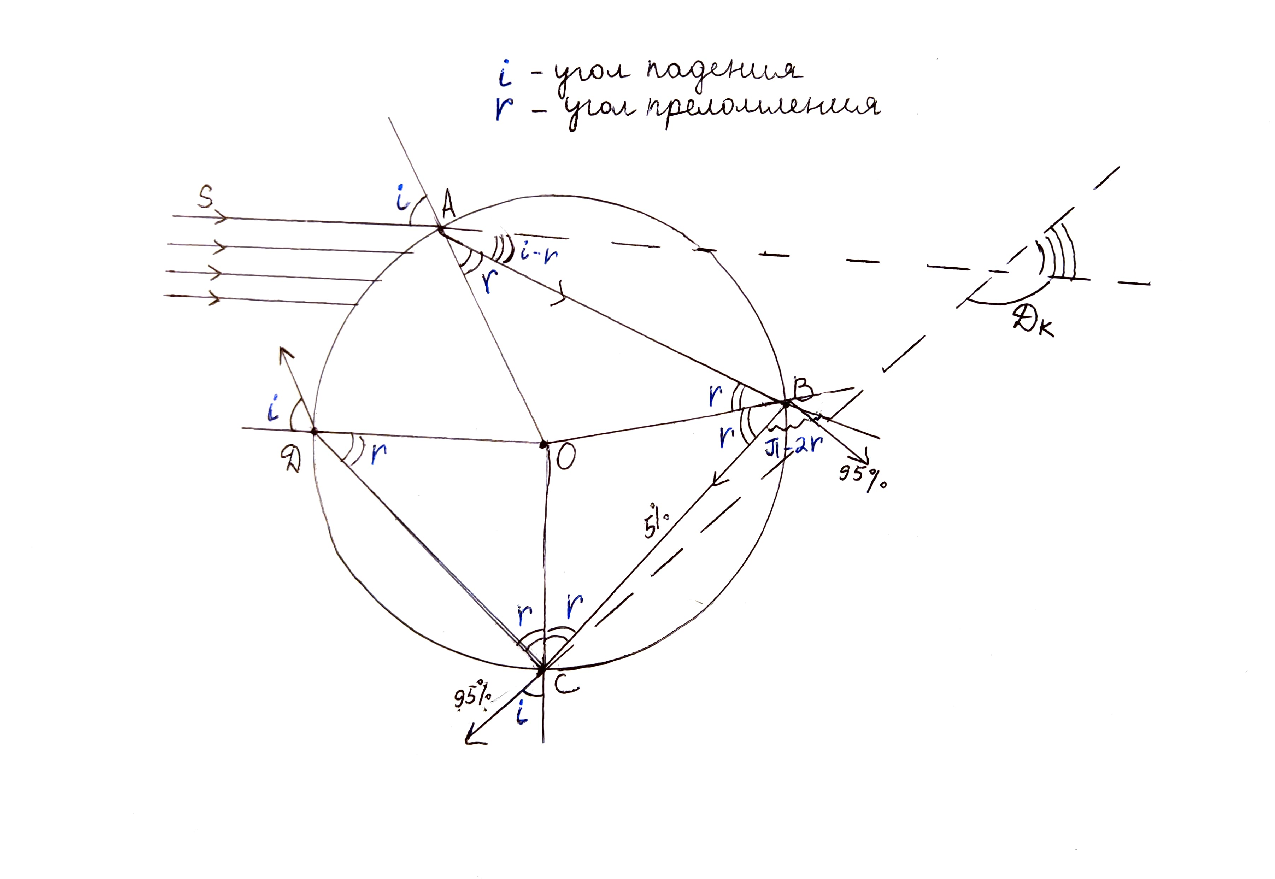
\includegraphics[width=8cm]{g1}\\
\textit{Рис.1. Ход светового луча в капле при образовании первой и второй радуг}\\

Пусть параллельный пучок солнечных лучей падает на каплю. Из-за кривизны поверхности капли, у разных лучей будут разные углы падения, поэтому угол падения $i \in [0^{\circ},90^{\circ}]$.\\ Рассмотрим некоторый луч, падающий в точку А под углом $i$. Преломившись с углом $r$, луч входит в каплю и достигает точки В. Часть энергии луча, преломившись, выходит из капли, часть, испытав внутреннее отражение в точке В, достигает точки С. Здесь снова часть энергии луча, преломившись. выходит из капли, а часть испытывает внутреннее отражение, переместившись в точку О. Внутренних отражений в капле может быть большое количество, а преломлений в капле всего два - на выходе и на входе.\\
Исходя из значений коэффициентов отражения для различных углов падения воды:\\
\begin{center}
\begin{tabular}{|l|l|l|l|l|l|l|}
\hline
$i$, $^{\circ}C$ & 0 & 20 & 40 & 60 & 80 & 90\\
\hline
$p$, $\%$ & 2 & 2,1 & 2,5 & 6 & 34,5 & 100\\
\hline
\end{tabular}
\end{center}
\textit{Таблица 1. Зависимость коэффициента отражения от угла падения}\\
где $i$ - угол падения, $p$ - коэффициент отражения\\
Видно, что большинство лучей будет преломляться.\\
При каждом отражении интенсивность убывает примерно в $$(\frac{n+1}{n-1})^2 \approx 50 \; \; \textit{раз}$$
Обозначим через $D_k$ угол, смежный к углу отклонения любого луча после прохождения им капли. Из рис.1 видно, что 
\begin{equation}
D_1 = 2(i - r) + \pi - 2r
\label{short}
\end{equation}
Параллельный пучок лучей, падающих на каплю, по выходе из капли оказывается сильно расходящимся. Концентрация лучей, а значит, их интенсивность тем больше, чем ближе они лежат к лучу, испытавшему минимальное отклонение. Только минимально отклоненный луч и самые близкие к нему лучи обладают достаточной интенсивностью, чтобы образовать радугу. Поэтому этот луч и называют \textit{лучом радуги}.\\

Минимальное отклонение луча, испытавшего одно внутреннее отражение $(k = 1)$, равно:
\begin{equation}
D_1 = 2(i - r) + \pi  - 2r = \pi + 2(i - 2r)
\label{short}
\end{equation}
Каждый белый луч, преломляясь в капле, разлагается в спектр, и из капли
выходит пучок расходящихся цветных лучей. Поскольку у красных лучей показатель преломления меньше, чем у других цветных лучей, то они и будут испытывать минимальное отклонение по сравнению с остальными.\\
\item \textbf{Угловая дисперсия радуги}\\
Используя выражение (2), закон преломления и зная, что $D_1$ должен быть максимальным (у луча радуги отклоняются минимально), найдем значение угла падения для различных компонент спектра. 
\begin{equation}
(D_1)' = (\pi + 2(i - 2r))' = 0
\label{short}
\end{equation}
\begin{equation}
\sin i = n \sin r
\label{short}
\end{equation}
Тогда:
\begin{equation}
(\pi + 2(\arcsin(n\sin r) - 2r))' = 0 
\label{short}
\end{equation}
\begin{equation}
-4 + \frac{2n \cos r}{\sqrt{1 - n^2 \sin^2 r}} = 0
\label{short}
\end{equation}
Откуда зависимость угла преломления луча радуги от коэффициента преломления выражается как:
\begin{equation}
\sin r = \sqrt{\frac{4 - n(\lambda)^2}{3n(\lambda)^2}}
\label{short}
\end{equation}
Воспользуемся табличными значениями зависимости коэффициента преломления воды при $20^{\circ}$ от длины волны $n(\lambda)$:
\begin{center}
\begin{tabular}{|l|l|l|l|}
\hline
$\lambda$, нм & n & $\lambda$, нм & n\\
\hline
1256,0 & 1,3210 & 508,6 & 1,3360\\
\hline
678,0 & 1,3308 & 486,1(F) & 1,3371\\
\hline
656,3 (C) & 1,3311 & 480,0 & 1,3374\\
\hline
643,8 & 1,3314 & 434,0 (G) & 1,3403\\
\hline
589,3 (D) & 1,3330 & 303,4 & 1,3581\\
\hline
546,1 & 1,3345 & 214,4 & 1,4032\\
\hline
\end{tabular}
\end{center}
\textit{Таблица 2. Зависимость показателя преломления от длины волны}\\
Откуда найдем углы падения, преломления и отклонения лучей радуги для красной (C), жёлтой (D), голубой (F) и синей (G) линий спектра:
\begin{center}
\footnotesize
\begin{tabular}{|l|l|l|l|l|}
\hline
угол & $656,3$ нм & $589,3$ нм & $486,1$ нм & $434,0$ нм\\
\hline
$r$, $^{\circ}C$  & 40,350 & 40,225 & 39,958 & 39,750\\
\hline 
$i$, $^{\circ}C$ & 59,521 & 59,410 & 59,172 & 58,987\\
\hline
$D_1$,$^{\circ}C$ & 137,642 & 137,92 & 138,512 & 138,974\\
\hline
$\pi - D_1$, $^{\circ}C$ & 42,358 & 42,08 & 41,488 & 41,026\\
\hline  
\end{tabular}
\end{center}
\textit{ Таблица 3. Углы первой радуги для различных длин волн}\\
\\
Угловая дисперсия рассчитывается по формуле:
\begin{equation}
D = \frac{d\theta}{d\lambda}
\label{short}
\end{equation}
Рассчитаем угловую дисперсию для двух близких (с точки зрения радуги) линий спектра - голубой и синей:
\begin{equation}
D_2 = \frac{0,462^{\circ}}{52,1 \; \textit{нм}} \approx 8,87 \cdot 10^6 \; \; \frac{\textit{град.}}{\textit{м}}
\label{short}
\end{equation}
Угловая ширина первой радуги составляет:
\begin{equation}
\triangle_1 = 42,358^{\circ} - 41,026^{\circ} = 1,332^{\circ} 
\label{short}
\end{equation}
\item \textbf{Вторая радуга и следующие}\\
Если повторить предыдущие рассуждения относительно лучей, испытавших в капле два внутренних отражения, получим следующие минимальные углы отклонения крайних цветных лучей:
\begin{equation}
D_2 = 6r - 2i
\label{short}
\end{equation}
Условие на угол преломления луча радуги:
\begin{equation}
\sin r = \sqrt{\frac{9 - n(\lambda)^2}{8n(\lambda)^2}}
\label{short}
\end{equation}
\begin{center}
\footnotesize
\begin{tabular}{|l|l|l|l|l|}
\hline
угол & $656,3$ нм & $589,3$ нм & $486,1$ нм & $434,0$ нм\\
\hline
$r$, $^{\circ}C$  & 45,570 & 45,466 & 45,244 & 45,072\\
\hline 
$i$, $^{\circ}C$ & 71,904 & 71,843 & 71,711 & 71,608\\
\hline
$D_1$,$^{\circ}C$ & 129,612 & 129,110 & 128,042 & 127,216\\
\hline
$\pi - D_1$, $^{\circ}C$ & 50,388 & 50,890 & 51,958 & 52,784\\
\hline  
\end{tabular}
\end{center}
\textit{ Таблица 4. Углы второй радуги для различных длин волн}\\
\\
Угловая дисперсия для двух близких (с точки зрения радуги) линий спектра - голубой и синей:
\begin{equation}
D_2 = \frac{0,826^{\circ}}{52,1 \; \textit{нм}} \approx 15,85 \cdot 10^6 \; \; \frac{\textit{град.}}{\textit{м}}
\label{short}
\end{equation}
Угловая ширина второй радуги составляет:
\begin{equation}
\triangle_2 = 52,784^{\circ} - 50,388^{\circ} = 2,396^{\circ} 
\label{short}
\end{equation}
Из таблицы 4 видно, что теперь наибольший угол отклонения имеет фиолетовая компонента, в то время как в первой радуге наибольший угол отклонения имела красная компонента. Это объясняет инвертированный порядок второй радуги: внешняя дуга второй радуги фиолетовая, а внутренняя - красная.\\
\\
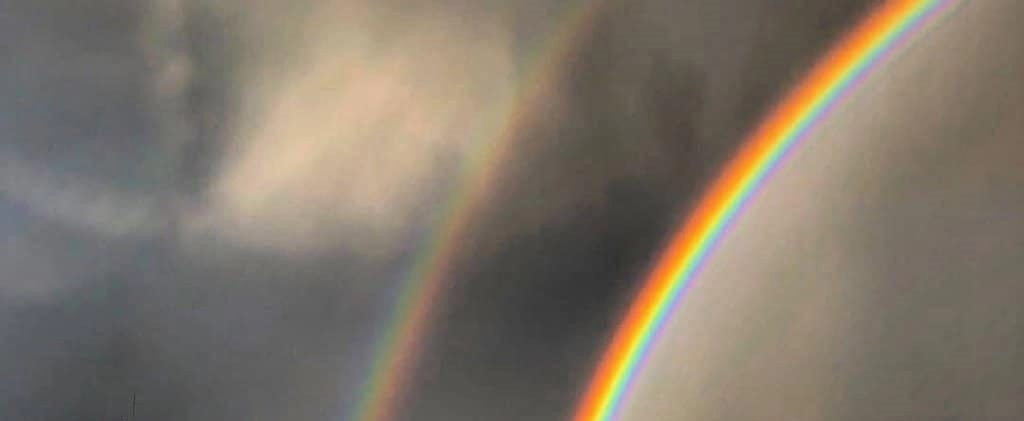
\includegraphics[width=8.5cm]{g2}\\
\textit{Рис.2. Пример двойной радуги}\\
При большем количестве отражений интенсивность становится очень маленькой, поэтому радугу порядка, выше второго, человеческим глазом увидеть очень сложно. \\
\item \textbf{Влияние размера и формы капель на вид радуги}\\
Расчеты по формулам дифракционной теории, выполненные для капель разного размера, показали, что весь вид радуги – ширина дуг, наличие, расположение и яркость отдельных цветовых тонов, положение дополнительных дуг
очень сильно зависят от размера капель дождя. Приведем основные характеристики внешнего вида радуги для капель разных радиусов.\\
\textit{Радиус капель 0,5-1 мм.} Наружный край основной радуги яркий, темнокрасный, за ним идет светло-красный, и далее чередуются все цвета радуги.
Особенно яркими кажутся фиолетовый и зеленый. Дополнительных дуг много
(до пяти), в них чередуются фиолетово-розовые тона с зелеными. Дополнительные дуги непосредственно примыкают к основным радугам.\\
\textit{Радиус капель 0,25 мм.} Красный кран радуги стал слабее. Остальные цвета
видны по-прежнему. Несколько фиолетово-розовых дополнительных дуг сменяются зелеными.
Радиус капель 0,10-0,15 мм. Красного цвета в основной радуге больше нет.
Наружный край радуги оранжевый. В остальном радуга хорошо развита. Дополнительные дуги становятся все более желтыми. Между ними и между основной радугой и первой дополнительной появились просветы.\\
\textit{Радиус капель 0,04-0,05 мм.} Радуга стала заметно шире и бледнее. Наружный край ее бледно-желтый. Самым ярким является фиолетовый цвет. Первая
дополнительная дуга отделена от основной радуги довольно широким промежутком, цвет ее белесый, чуть зеленоватый и беловато-фиолетовый.\\
\textit{Радиус капель 0,03 мм}. Основная радуга еще более широкая с очень слабо
окрашенным чуть желтоватым краем, содержит отдельные белые полосы.\\
\textit{Радиус капель 0,025 мм и менее}. Радуга стала совсем белой. Она примерно в
два раза шире обычной радуги и имеет вид блестящей белой полосы. Внутри
нее могут быть дополнительные окрашенные дуги, сначала бледно-голубые или
зеленые, затем белесовато-красные.\\
\\
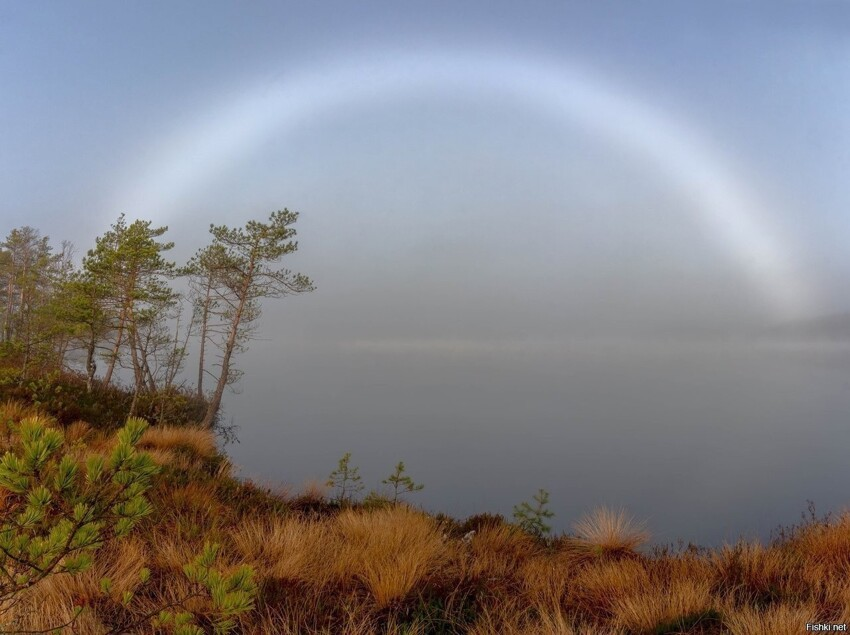
\includegraphics[width=8.5cm]{g3}\\
\textit{Рис.3. Белая радуга}\\
\end{enumerate}
\end{multicols}
\end{document}